%\documentclass[10pt,twocolumn]{article}

%\usepackage{graphicx, color}
%\usepackage[font=small,labelfont=bf]{caption}
%\usepackage[subrefformat=parens]{subcaption}
%\usepackage{amsmath}
%\usepackage{subcaption}
%\usepackage{url}
%\usepackage{listings}

%\begin{document}

%\title{Finding An Unified Programming Model for Future Network Functions}

%\maketitle

%\section{Background and Motivation}

In recent years, the research community has witnessed the quick development of
network function virtualization (NFV). DPDK \cite{dpdk} and Netmap
\cite{rizzo2012netmap} use kernel bypassing to speed up the performance of NF
software. They have become the default libraries for implementing high-speed
modern NF software. NFV management systems such as E2 \cite{palkar2015e2} are
built to dynamically scale virtual instances running different NFs. NFs are
augmented with fault tolerance \cite{sherry2015rollback} and flow migration
\cite{gember2014opennf} to improve the failure resilience.

However, despite all these advancements, a core problem is not well-solved by
existing work: what should be the default programming abstraction for implementing NF
software, so that the diverse requirements of NF software can be well-captured
by this abstraction? To show the importance of this problem, let me first discuss
the diversity of NF software.

\subsection{Diversity of NF Software}


\noindent \textbf{Simple Packet Processing Program.} Example NFs include
firewall, NAT and load balancer. The word ``simple'' actually means that the way
that these NFs manipulate packets is simple: they take an input packet,
perform necessary packet transformation and book-keeping, then they release the
packet to the outside. Taking NAT as an example. After receiving an input
packet, NAT may update the connection status associated with the flow, then the
NAT performs an address translation to substitute the IP address and port of the
packet. Finally, NAT sends the packet out from the output port.

\textit{These NFs can be effectively implemented inside a polling loop and can be
seamlessly integrated with either DPDK or Netmap for maximum performance.}

\noindent \textbf{NFs with Intensive File I/O.} Example NFs include PRADs
\cite{prads} asset monitor and Snort \cite{snort} intrusion detection system
(IDS). For instance, PRADS is a passive real-time asset detection system, which
listens to network traffic and logs important information on hosts and services
it sees on the network. This information can be used to map the underlying
network, letting network operators know what services and hosts are active, and
can be used together with IDS/IPS setup for "event to application" correlation.

Both PRADs and Snort can be ported to use DPDK to speed up packet processing
\cite{201546}. Even after porting to DPDK, both NFs fail to achieve 10Gbps line
rate processing \cite{201546}. The primary reason for this undesirable number is
due to logging. After porting to DPDK, the worker threads of both NFs keep
polling for new packets and maintain CPU usage to 100\%. But when both NFs log
important events, they have to access system calls related to file system
processing, generating expensive context switches and compromising the packet
processing throughput.

\textit{These NFs can be accelerated using DPDK and Netmap, but they still need
  to step into the kernel to log events to the files.} NFs with intensive file
I/O remain to be interesting phenomena in existing NFV research. People have
strived to remove context switches associated with kernel networking stack by
bypassing the kernel with DPDK, but they fail to remove the context switches
associated with kernel file systems during logging.

\noindent \textbf{NFs with Reliable Communication to External Services.}
Example NFs include S-CSCF in IMS system \cite{3gpp-ims} and NFs that need to
replicate their states on back NFs.

S-CSCF is an important middlebox sitting at control plane of the IMS system. It
processes SIP \cite{sip} messages by contacting several external
services. Taking the S-CSCF implementation of a famous open source IMS project
Clearwater \cite{project-clearwater} as an example, when processing SIP messages,
S-CSCF needs to log SIP registration information on a Memcached \cite{memcached}
cluster and acquire user information by querying a dedicated storage server
called Home Subscriber Server (HSS). The S-CSCF implementation of Clearwater
uses kernel TCP/IP stack to carry out reliable communication to all the required
external services, seriously limiting the maximum throughput that S-CSCF can
achieve. Our experience with Clearwater shows that a single worker thread in
S-CSCF can only process SIP messages with the bandwidth of 40Mb.

FTMB \cite{sherry2015rollback} is the state of art system for NF replication. It
employs a primary-backup replication strategy. On the primary NF instance,
after each packet is processed, the packet is passed to the backup over a
reliable communication channel for replication. We can treat the replication
process as communicating external services: each input packet processed by the
primary instance must be reliably delivered to the backup instance. FTMB uses
DPDK to speed up packet processing and implements its own reliable communication
channel on top of DPDK. But the implementation detail of the reliable
communication channel is omitted from the paper. It would be desirable to
implement the reliable communication channel using a user-level TCP/IP stack
like mTCP \cite{179773}, so that the performance of FTMB is stable (a
handcrafted reliable communication channel may be unstable and lack of flow
control) and it is easier to reproduce FTMB implementation for both academic and
industrial usage. \textit{However, without a good programming abstraction,
  integrating a user-level TCP implementation like mTCP with replication
  strategy like FTMB is not a trivial task:} mTCP exposes an event-driven
programming interface like Linux epoll. The application thread using mTCP does
not sit in the same thread as the mTCP worker thread. But FTMB requires that the
same worker thread handles both NF packet processing and reliable communication
to ensure correct replication.

\textit{Some of these NFs abandoned DPDK
  and Netmap, use kernel networking stack to provide reliable communication
  channel, but sacrifice performance. Some of these NFs use DPDK and Netmap to
  speed up packet processing and implement their own reliable communication
  channel, but sacrifice the stable performance and flow control provided by TCP/IP. }



\noindent \textbf{NFs that Process Events Raised by Lower-level System
  Components.} Example NFs include Snort IDS \cite{snort} and Bro IDS
\cite{bro}. The two IDSes alert potential attacks by matching the flow protocols
and analyzing flow payloads with an automaton. They can be decoupled into two
parts: A low-level system is responsible for re-assembling the TCP stream and
generating events associated with the TCP stream, i.e. connection setup,
packet re-transmission, and the new packet payload. A high-level event driven
system is responsible for reacting to the events raised by the low-level system,
i.e. in the case of a fake re-transmission forged by an attacker, the IDS drops the
flow and raises an alert. These IDSes can be effectively accelerated using mOS
\cite{201546}, which substitute the low-level system that raises flow-related
events. mOS is accelerated using DPDK and is an improved version of mTCP \cite{179773}.

\textit{The low-level system of these NFs can be accelerated with DPDK. However,
  the low-level system like mOS is usually targeted to process TCP/IP protocol
  and can not be extended to process non-TCP/IP protocol.}

\noindent \textbf{Summary.} Now we briefly discuss the similarities and
differences of all the discussed NF software.

\noindent \textbf{Similarity.} Most of these NFs can be accelerated with DPDK or
Netmap (except for S-CSCF, which relies on kernel networking stack, but we can
still accelerate it by porting it to user-level TCP/IP stack like mTCP). Using
DPDK or Netmap means that the worker threads in these NFs become busy polling
thread that keeps CPU usage to 100\%, implying that any system calls entering
the kernel context may compromise the performance of these NFs.

\noindent \textbf{Difference.} These NFs have different working goals and
operate at different levels. Simple packet processing programs only manipulate
raw packets. They do not rely on any external services. PRADs needs to do file
I/O. FTMB and S-CSCF need to communicate with external services. Snort and Bro
operate on a high-level that reacts to flow-level events raised by a low-level
system components. These differences lead to diverse implementation details,
making it hard to find an appropriate abstraction to unify these NFs. 

\subsection{One Abstraction to Rule Them All}

Just like the dedication that physicists put into the grand unified theory,
computer scientists also have been searching for a unified programming
abstraction that can capture a variety of applications. In terms of NFV, if a
unified programming abstraction can be found for all the NFs mentioned in
the previous section, programmers can enjoy the following benefits.

First, by optimizing the performance of the library that provides the
unified programming abstraction, we can improve the performance for a huge variety of
NFs. There is no need to optimize each NF, which might take a huge amount of
labor work.

Second, ease NF software development. Once the implementor becomes familiar with
the programming abstraction, he is able to create different types of NFs without
learning different programming paradigms or constructing different libraries.

Finally, it makes important research and industrial result easily reproducible,
as the unified programming abstraction makes people play on the same ground.

Such a programming abstraction is readily accessible for NFV implementors and
researchers, which is functional reactive programming, especially the subset
related to futures, promises and continuations.

\subsection{Futures and Promises}

Futures and promises are important terminologies in functional reactive
programming. A future represents a value that is going to be computed while a
promise represents the action when the computation is done. This simple
programming paradigm can easily capture most of the asynchronous programming
patterns. Let me briefly explain how futures and promises can be mapped to NFs
discussed in previous sections.

For simple packet processing program, the futures are packets that are going to
be received whereas the promises are packet handler functions.

For PRADs, the futures and promises can be combined to implement efficient file
system logging. The futures represent the logging action that will log events
raised by PRADs to the file system. The promises represents post actions when
the logging is done.

For S-CSCF and FTMB, futures and promises can be used to implement an efficient
user-space TCP/IP stack. The futures are still packets to be received, but the
promises become TCP/IP stack handlers.

For Snort and Bro, futures and promises can be used to implement a low-level
system that raises flow events. Futures flow events that are going to be raised,
promises are event handlers for these events.

The future-promise programming abstraction can be efficiently implemented with
a small runtime overhead (i.e. asynchronous C++ library Seastar
\cite{seastar}). The programming abstraction can fully bypass the entire kernel,
even in terms of file logging (with the help of DMA), providing satisfactory
performance for modern NF software.

\subsection{Contribution}

In this paper, we are going to make the following contributions.

First, we are the first to apply functional reactive programming as a generic
method for building a variety of NF software. We use seastar as the underlying
library for providing the reactive programming abstraction.

Second, we carry out case studies to show how functional reactive programming
can be used to construct 4 different types of NFs, with diverse requirements.

Finally, we show that the performance and ease of implementation are greatly
improved by using functional reactive programming. In particular:

\noindent \textbf{We re-implement PRADs using functional reactive programming.}
The resulting PRADs is capable of logging to file system at a throughput of
several gigabits per second.

\noindent \textbf{We create a new primary-backup replication strategy.} The new
primary-backup strategy is capable of processing packets at line rate. The
biggest difference between this replication strategy with FTMB is that it does
not need to checkpoint the master NF instance, greatly simplifying the
implementation effort. It has no replay time and introduces no extra latency
caused by checkpointing.

\noindent \textbf{We re-implement mOS using our new programming abstraction.} We
also port PRADs to use the new mOS and show that the new PRADs can be several
times faster than that in the mOS paper \cite{201546}.


%\section{Primary-backup NF Replication Without Rolling Back}
%To be continued.

%\section{Rollback Recovery for Middleboxes}

\subsection{FTMB and Non-determinism in Multi-threaded NF}

FTMB \cite{sherry2015rollback} is the state-of-art middlebox replication
strategy. FTMB regularly creates a checkpoint for the primary NF instance and
generates a series of packet access logs. In the case of primary NF instance
failure, FTMB recover the primary NF instance by rollback: a new primary NF
instance is re-created based on the latest checkpoint and the state of the new
primary NF instance is recovered by replaying the packet access log. 


FTMB simply rejected the idea to keep the primary NF instance and the backup NF
instance synchronized, due to the exsitence of shared variables and
non-determinism caused by concurrently accessing shared variables.

A multi-threaded NF software may maintain several shared variables, protected by
locks. Accessing these shared variables from multiple worker threads may result in
non-determinism: when the same input sequence are fed into two identical
programs, they may fail to generate the same output.

For instance, the NF software maintain a shared variable $v$. There are two NF
instances running the same NF software. Both NF instances are configured with
two worker threads $t_1$ and $t_2$. Then, two identical packets $p_1$ and $p_2$
are concurrently fed into worker threads $t_1$ and $t_2$ respectively, on both
of the two NF instances. Because the two worker threads run in parrallel, it is
impossible to guarantee the order for accessing the shared variable $v$. We
might end-up with the following situation: on the first NF instance, $t_1$ first
accesses $v$ when processing $p_1$, while on the second NF instance, $t_2$ first
accesses $v$ when processing $p_2$. This situation may render the two identical
NF instances to be in different states.

Due to the non-determinism, the authors of FTMB \cite{sherry2015rollback} reject
the design to keep primary and backup synchronized: without tagging the packet
processing order from the master instance, it is impossible to keep the backup
instance synchronized. Even if master instance correctly tags the packet
processing order and sends these tags to the backup instance, the worker threads
on backup instance must strictly follow the packet processing order when
accessing the shared variable: before accessing a shared variable, the worker
thread must keep spinning to wait for its turn to access the shared variable,
compromising the performance of the backup instance.

\subsection{Execution Model of FTMB}

FTMB uses rollback recovery, which could be summarized as follows: the primary
instance create a \textbf{Packet Access Log}(PAL for short) whenever accessing a
shared variable. For each processed packet, the primary instance sends the
processed packet, together with all the PALs generated during processing this
packet, to the backup instance over a reliable communication channel. The backup
instance in FTMB is actually referred to as a \textbf{Output Logger}. The output
logger stores the PALs for rollback recovery and release the processed packet to
the outside. In the meantime, since the primary instance runs in a virtual
machine, the primary instance also sends a checkpoint of its virtual machine
state to the output logger. The output logger saves the current checkpoint,
discards the previous checkpoint and all the PALs received since the previous
checkpoint.

If the primary instance crashes, the primary instance is recovered as follow:
the output logger uses the saved checkpoint of the primary instance to create a
new virtual machine. Then the output logger sends the PALs and the input packets
that trigger the generation of these PALs to the new primary instance for
replay. The primary instance resumes working after it finishes replaying all the
PALs.

\subsection{Pros and Cons of FTMB}

Pros:

\textbf{Good system performance.} FTMB is carefully designed not to introduce
small overhead when generating PALs. The replicated NF in FTMB is able to
processes millions of packets per second.

\textbf{Fast recovery time.} Depending on how often the primary instance is
checkpointed, the recovery time in the case of primary failure can be as small
as 20 milliseconds.

\textbf{Passive Operation.} There is no dedicated backup instance in
FTMB. The output logger is capable of relicating multiple primary instances.

\noindent Cons:

\textbf{Packet processing latency is increased during checkpoint.} When doing
checkpoint for primary instance, the primary instance is significantly slowed
down, resulting in packet processing latency up to several milliseconds. This
leads to a huge jitter in the network RTT, which may be devastating to some
important applications such as VoIP and on-line gaming.

\textbf{The tradeoff between packet latency and checkpoint frequency.} An
important parameter to tune in FTMB is how frequently should the primary
instance be checkpointed. If the primary instance is frequently checkpointed,
then the recovery time would be faster, but each time when checkpoint is
triggered, FTMB adds huge packet processing latency, sometimes up to several
milliseconds. If the primary instance is not frequently checkpointed, then the
output logger needs a huge buffer to buffer input packets and PAL, the recovery
time is also prolonged.

\textbf{Lacking An Open-souce Solution.} FTMB is a very complicated system,
involving several critical system components that are non-trivial to
engineer. However, FTMB is not open-sourced and therefore limititing its further
application in both academia and industry.



%%\section{Asynchronous Programming}
%The core idea of asynchronous programming is to handle all the tasks that need
%to block waiting for results asynchronously, so that nothing is really blocked.

%It can be implemented using an active poll loop. The active poll loop polls
%different event source for events. Whenever an event happens, the poll loop
%executes a callback function associated with the event to handle the event.

%An improved asynchronous programming style is to use futures and promises. The
%future and promise abstraction can handle asynchronous programming in a nice
%manner.

%Asynchronous programming is the solution for all the problems that I have
%mentioned in the previous section.

%\section{Seastar and OSv}

%Seastar is a modern asynchronous programming library with future and promise
%style. It can be combined together with DPDK to achieve low-level packets
%processing. It also includes a user-space TCP/IP stack that is driven by
%asynchronous programming.

%It is the best asynchronous programming library that we can use to build network
%functions.

%Seastar can also run in OSv, a unikernel. In this way we can achieve
%high-performance virtualization.

%\section{Planned Roadmap}

%I plan to do the following case studies using Seastar in this work.

%First, implementing an unified NFV platform like NetBricks. Highlight that with
%the help of C++ unique\_ptrs, we can achieve the similar software memory safety
%like NetBricks.

%Second, port PRADS to use Seastar. Show that with the help of asynchronous
%programming, we can greatly improve the performance of PRADS.

%Third, implement a simplified version of mOS. Show that asynchronous programming
%can greatly simplify flow event generation and processing.

%Fourth, re-implement FTMB. Show that how easy it is to implement primary-backup
%replication for network functions using seastar.

%Fifth, a simplified SDN switch using Seastar, show it's performance boost when
%compared against OpenVSwitch.

\section{Promises and Cooperative Threads}

In this section, I will first give a detailed overview about promises and
cooperative threads used by Seastar fraemwork. Then I will introduce how to
apply promises and coopeartive threads to NFV.

\subsection{Lwt}

The core building blocks of Seastar are promises and cooperative
threads. Clearly, these fancy concepts come from the world of functional
programming languages. There is an Ocaml library called Lwt \cite{vouillon2008lwt}, which also
implements promises and cooperative threads. In the following sections, I will
first discuss how promises and coopeartive threads are implemented in
Ocaml. Then I will show how they are implemented in Seastar.

\subsubsection{Lwt Overview}

When wring programs like network servers, non-blocking is a very important
property that ensures the runtime efficiency of the network servers. There are
two dominant techniques to make the program non-blocking. The first one uses
multi-threading to support non-blocking, i.e. whenever a blocking operation is
going to be made, the main thread of the program lanuches another thread to
handle the blocking operation. The second one uses event-based programming
method, i.e. the main thread treats the completion of the blocking operation as
an event and register corresponding event handlers to handle this event.

The first technique is easy to use and easy to program. The program can be
written in traditonal way without relying on callbacks. However, the first
technique lacks efficiency, as launching too many threads compromises the
runtime performance. On the other hand, the second technique has superior
runtime performance, as it only maintains a single thread. However, it is
difficult to write programs using the second technique due to excessive use of
callbacks.

Lwt uses promises and cooperative threads to support non-blocking. The runtime
performance of Lwt is very good, as it only maintains a single physical thread
like the second technique. And it is quite easy to use. Writing asynchrounous,
fully non-blocking programs using Lwt is just like writing synchronous, blocking
programs using the first technique.

%\verb!sdfs\_dff!

%\begin{verbatim}
%Text enclosed inside environment
%is printed directly
%and all \LaTeX{} commands are ignored.
%\end{verbatim}

In the following sections, to facilitate understanding, I simplify some concepts
related with exception handling and modify the name of some important types in
Lwt.

\subsubsection{Promise State}

\begin{figure}[!h]
        \centering
        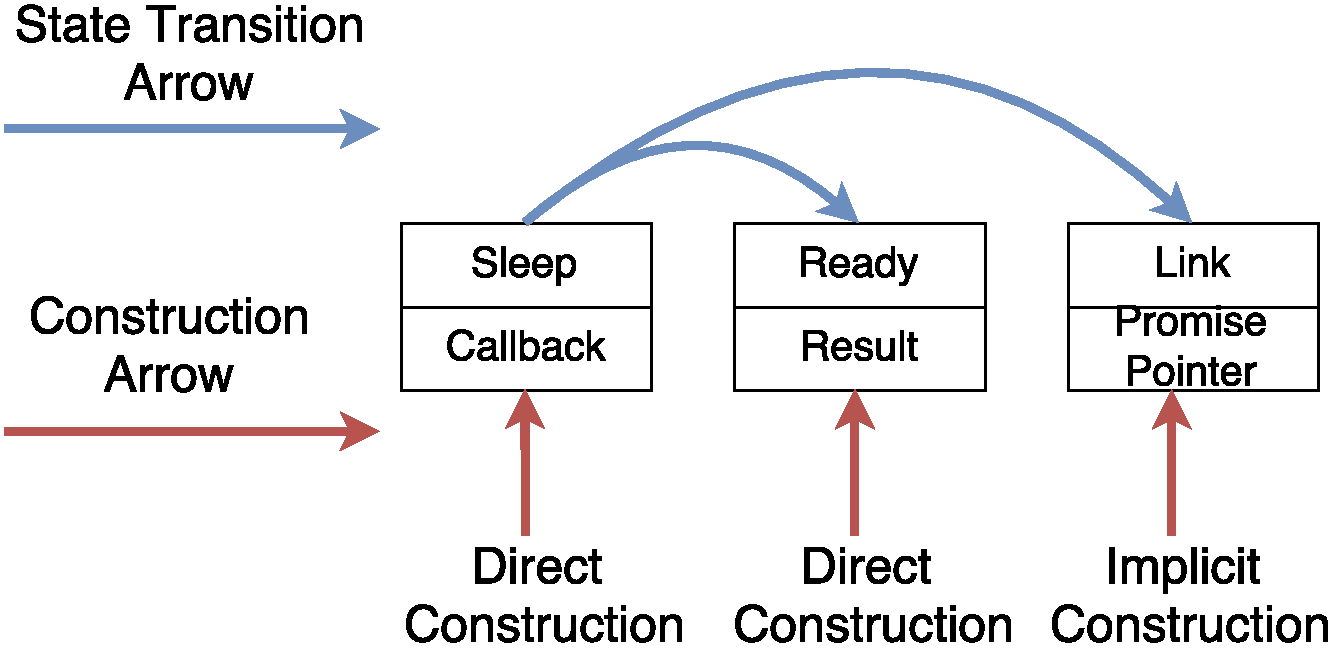
\includegraphics[width=1\columnwidth]{figure/promise-state.pdf}
        \caption{The state of a promise. The blue arrow represents how future
          states are transitioned. The red arrow represens whether can a
          programmer construct a certain state.}
        \label{fig:promise-state}
\end{figure}

The basic building block in Lwt is promise. A promise, as shown in figure
\ref{fig:promise-state}, has three states, which are \textbf{Sleep} state,
\textbf{Ready} state and \textbf{Link} state. The \textbf{Sleep} state
represents that the result of the promise is not available yet and one has to
wait before the \textbf{Sleep} state transitions into \textbf{Ready} state. The
\textbf{Sleep} state promise may contain a callback function, which is
immediately called after it is transitioned to \textbf{Ready}
state. \textbf{Ready} state represents that the result is available and we can
peek the result by checking the result field. Finally, the \textbf{Link} state
contains a pointer to a promise that is in \textbf{Sleep} state. It is used to
when waiting for multiple events.

The state of a proimse can be changed. The blue arrow of figure
\ref{fig:promise-state} shows the state transition graph between the three
states. Only \textbf{Sleep} state can generate a state transition.

When programming with promises, the programmer can only construct \textbf{Sleep}
state promise and \textbf{Ready} state promise. The \textbf{Link} state promise
is implicited constructed when chaining a promise with an annoynamous function
(we omit the discussion, as it does not affect the understanding of how promises
work).

\subsubsection{Chaining Promises}

\begin{verbbox}(>>=) : Promise a -> (a -> Promise b) -> Promise b \end{verbbox}

\begin{figure}[!h]
\resizebox{0.95\columnwidth}{!}{\theverbbox}
\caption{The infix operator for chaining promises.}
\label{fig:infix}
\end{figure}



Multiple promises can be chained together to accomplish complicated
tasks. Chaining is done through an infix operator \verb!>>=! (the then member
function of future in Seastar) as shown in figure \ref{fig:infix}, whose
signature is listed below.

Here, \verb!Promise a! represents a promise that, when transitioning into
\textbf{Ready} state, contains a result field with type \verb!a!. \verb!(a -> Promise b)!
represents an annouymous function, that takes a value of type \verb!a! as
argument and returns a value with type \verb!Promise b!. \verb!>>=! is a
function, that takes a value of \verb!Promise a! and an anouymous function of
\verb!(a -> Promise b)! and returns a value of \verb!Promise b!.

The real power of the \verb!>>=! operator is to chain multiple promises together
into a complicated operation. We give a piece of example code in figure
\ref{fig:example}. The code will first sleep for 3 seconds, then print "first
print" on the screen, then sleep another 3 seconds, and finally print "second
print" on the scrren. The best thing about this code is that, even if it
represents the consecutive execution of four blocking operations, but the code
itself is not blocking at all. It will return a promise in \textbf{Sleep} state
after being called. The blocking operations are implicitly handled by a
background thread.

\begin{verbbox}
  sleep 3 >>=
  fun () -> async_print "first print" >>=
  fun () -> sleep 3 >>=
  fun () -> async_print "second print"
\end{verbbox}

\begin{figure}[!h]
\resizebox{0.95\columnwidth}{!}{\theverbbox}
\caption{Chaining multiple promises into a complicated operation. The code above
  will first sleep for 3 seconds, then print "first print" on the screen, then
  sleep another 3 seconds, and finally print "second print" on the scrren.} 
\label{fig:example}
\end{figure}

\subsubsection{Annatomy of the infix operator}

\begin{verbbox}
(>>=) x f =
  match x with
  | Result r -> f r
  | Sleep ->
    let res = make_Sleep_promise () in
    add_callback x ( fun x -> connect res (x >>= f) )
    res
  | Link p ->
    assert false

connect t t' =
  match t' with
  | Result r -> (run t's callback)
  | Sleep ->
    (let t' link to t)
  
\end{verbbox}
\begin{figure}[!h]
\resizebox{0.95\columnwidth}{!}{\theverbbox}
\caption{The implementation of the infix operator. } %Depending on the state of the
  %promise \verb!x!, \verb!>>=! steps into three branches. If \verb!x! is a
 %result promise, then the annoynamous function.}
\label{fig:infix-internal}
\end{figure}

\noindent \textbf{The internal of the infix operator.} Depending on the state of
promise \verb!x!, the infix operator may step into two branches. If \verb!x! is
in \textbf{Result} state, then the anonymous function is immediately
excuted. But if \verb!x! is in \textbf{Sleep} state, the operator first creates a new
promise \verb!res! in \textbf{Sleep} state. Then a callback is added to \verb!x!. When
\verb!x! becomes \textbf{Result} state, the callback function is called, which
connects \verb!res! and \verb!x >> f!. The \verb!connect! function means that
the state of promise \verb!t'! will be reflected in promise \verb!t!.

\noindent \textbf{A conceptual explanation.} When executing \verb!x >>= f!, if
\verb!x! is immediately available and in \textbf{Result} state, then the
execution of the anonymous function \verb!f! continues without any
interruption.

The tricky part comes when \verb!x! is in \textbf{Sleep} state. It implies that
the result of \verb!x! is going to be available in the future. To prevent the
infix operator from blocking, we construct a new \textbf{Sleep} state promise
\verb!res! and returns \verb!res! to the user. Apparently, \verb!res! should
reflect the actual result of \verb!x >>= f!. To achieve this, before returning
\verb!res! to the user, we add a callback function to \verb!x!, which manually
connect \verb!res! with \verb!x >>= f! when \verb!x! becomes ready. In this way,
we mannualy construct a fully non-blocking abstraction.


\subsubsection{Wake Up Sleep Promise}

If a promise is in \textbf{Sleep} state, it must be waken up in the future and
transform into \textbf{Result} state. This is done by an external polling thread
which polls asynchronous completion messages. If the blocking operation that a
\textbf{Sleep} promise waits for has completed, the corresponding promise is
waken up.

\subsection{Seastar}

Seastar is basically a re-implementation of lwt in C++. It differes from lwt:

\textit{First}, the infix operator \verb!>>=! that chains promises together becomes
\verb!then! member function.

\textit{Second}, Seastar introduces a new object called \verb!future!, which is actually
a pointer object to the underlying promise. The reason is that C++ has no
garbage collection and Seastar has to manually manage the the memory allocation
of the promise object. Currently, Seastar either allocates the promise object
directly on the heap, or captures the promise object inside the callback
function. Therefore, to query the promise, seastar creates a pointer object
future, which contains a pointer to the underlying promise object.


\subsection{Promises in NFV}

We use promises to hide any kind of blocking operations when processing
packets. We give some usage examples.

\subsubsection{Simple Packet Processing}

\begin{verbbox}
xxx.then([]{
  process packet;
  return new_future;
}).then([]{
  process packet;
  return new_future;
})
  
\end{verbbox}
\begin{figure}[!h]
\resizebox{0.5\columnwidth}{!}{\theverbbox}
\caption{Example code of a simple packet processing software.} 
\label{fig:spps}
\end{figure}

It is straightforward to implement a simple packet processing software using
promises, as shown in figure~\ref{fig:spps}. The multiple chained promises
represent multiple processing stages on a packet processing pipeline.

\subsubsection{Using Promises to Hide Blocking During File IO}

\begin{verbbox}
xxx.then([]{
  do file IO;
  return new_future;
}).then([]{
  resume packet processing;
  return new_future;
})
  
\end{verbbox}
\begin{figure}[!h]
\resizebox{0.5\columnwidth}{!}{\theverbbox}
\caption{Example code of a NF that performs file IO.} 
\label{fig:file-io}
\end{figure}

Figure \ref{fig:file-io} represents a NF that performs file IO in the middle of
packet processing. Previously, this incurs kernel context switches and blocking,
which may compromise the performance of the NF. But with promise, the kernel
context switches and blocking are hidden by the promises, making the entire
operation fully non-blocking.

After issuing \verb!do file IO!, the NF software can continue to process other
flows. When file IO finishes, the processing of the original packet that incur
the file IO is resumed. This can greatly boost the performance of NFs that need
to perform file IO, such as PRADs.

\subsubsection{Handling Shared Variable Accessing}

\begin{verbbox}
xxx.then([]{
  access shared variable;
  return new_future;
}).then([]{
  resume packet processing;
  return new_future;
})
  
\end{verbbox}
\begin{figure}[!h]
\resizebox{0.5\columnwidth}{!}{\theverbbox}
\caption{Example code of a NF that needs to access shared variable.} 
\label{fig:asv}
\end{figure}

Figure \ref{fig:asv} shows an example of how to use promise to handle shared
variable processing. After issuing \verb!access shared variable!, the processing
is temporarily suspended and a request is created and sent to another thread to
access the shared variable. After modifying the shared variable, the suspended
packet processing is resumed.

By using promises, we can effectively linearize shared variable
accessing. Therefore we can keep the primary NF instance and the backup NF
instance in the same state, which simplifies primary-backup replication even in
multi-threaded environment.




%\bibliographystyle{abbrv}
%\bibliography{Bibliography}

%\end{document}

% TEMPLATE for Usenix papers, specifically to meet requirements of
%  USENIX '05
% originally a template for producing IEEE-format articles using LaTeX.
%   written by Matthew Ward, CS Department, Worcester Polytechnic Institute.
% adapted by David Beazley for his excellent SWIG paper in Proceedings,
%   Tcl 96
% turned into a smartass generic template by De Clarke, with thanks to
%   both the above pioneers
% use at your own risk.  Complaints to /dev/null.
% make it two column with no page numbering, default is 10 point

% Munged by Fred Douglis <douglis@research.att.com> 10/97 to separate
% the .sty file from the LaTeX source template, so that people can
% more easily include the .sty file into an existing document.  Also
% changed to more closely follow the style guidelines as represented
% by the Word sample file. 

% Note that since 2010, USENIX does not require endnotes. If you want
% foot of page notes, don't include the endnotes package in the 
% usepackage command, below.

% This version uses the latex2e styles, not the very ancient 2.09 stuff.
\documentclass[letterpaper,twocolumn,10pt]{article}
\usepackage{usenix,epsfig,endnotes}

\usepackage{graphicx, color}
\usepackage[font=small,labelfont=bf]{caption}
\usepackage[subrefformat=parens]{subcaption}
\usepackage{amsmath}
\usepackage{subcaption}
\usepackage{url}
\usepackage{listings}
\usepackage{verbatimbox}

\begin{document}

%make title bold and 14 pt font (Latex default is non-bold, 16 pt)
\title{\Large \bf Liveraging Functional Reactive Programming to Build Modern NFV Applications}

\maketitle

\subsection*{Abstract}
Abstract

\section{Background and Motivation}

In recent years, the research community has witnessed the quick development of
network function virtualization (NFV). DPDK \cite{dpdk} and Netmap
\cite{rizzo2012netmap} use kernel bypassing to speed up the performance of NF
software. They have become the default libraries for implementing high-speed
modern NF software. NFV management systems such as E2 \cite{palkar2015e2} are
built to dynamically scale virtual instances running different NFs. NFs are
augmented with fault tolerance \cite{sherry2015rollback} and flow migration
\cite{gember2014opennf} to improve the failure resilience.

However, despite all these advancements, a core problem is not well-solved by
existing work: what should be the default programming abstraction for implementing NF
software, so that the diverse requirements of NF software can be well-captured
by this abstraction? To show the importance of this problem, let me first discuss
the diversity of NF software.

\subsection{Diversity of NF Software}


\noindent \textbf{Simple Packet Processing Program.} Example NFs include
firewall, NAT and load balancer. The word ``simple'' actually means that the way
that these NFs manipulate packets is simple: they take an input packet,
perform necessary packet transformation and book-keeping, then they release the
packet to the outside. Taking NAT as an example. After receiving an input
packet, NAT may update the connection status associated with the flow, then the
NAT performs an address translation to substitute the IP address and port of the
packet. Finally, NAT sends the packet out from the output port.

\textit{These NFs can be effectively implemented inside a polling loop and can be
seamlessly integrated with either DPDK or Netmap for maximum performance.}

\noindent \textbf{NFs with Intensive File I/O.} Example NFs include PRADs
\cite{prads} asset monitor and Snort \cite{snort} intrusion detection system
(IDS). For instance, PRADS is a passive real-time asset detection system, which
listens to network traffic and logs important information on hosts and services
it sees on the network. This information can be used to map the underlying
network, letting network operators know what services and hosts are active, and
can be used together with IDS/IPS setup for "event to application" correlation.

Both PRADs and Snort can be ported to use DPDK to speed up packet processing
\cite{201546}. Even after porting to DPDK, both NFs fail to achieve 10Gbps line
rate processing \cite{201546}. The primary reason for this undesirable number is
due to logging. After porting to DPDK, the worker threads of both NFs keep
polling for new packets and maintain CPU usage to 100\%. But when both NFs log
important events, they have to access system calls related to file system
processing, generating expensive context switches and compromising the packet
processing throughput.

\textit{These NFs can be accelerated using DPDK and Netmap, but they still need
  to step into the kernel to log events to the files.} NFs with intensive file
I/O remain to be interesting phenomena in existing NFV research. People have
strived to remove context switches associated with kernel networking stack by
bypassing the kernel with DPDK, but they fail to remove the context switches
associated with kernel file systems during logging.

\noindent \textbf{NFs with Reliable Communication to External Services.}
Example NFs include S-CSCF in IMS system \cite{3gpp-ims} and NFs that need to
replicate their states on back NFs.

S-CSCF is an important middlebox sitting at control plane of the IMS system. It
processes SIP \cite{sip} messages by contacting several external
services. Taking the S-CSCF implementation of a famous open source IMS project
Clearwater \cite{project-clearwater} as an example, when processing SIP messages,
S-CSCF needs to log SIP registration information on a Memcached \cite{memcached}
cluster and acquire user information by querying a dedicated storage server
called Home Subscriber Server (HSS). The S-CSCF implementation of Clearwater
uses kernel TCP/IP stack to carry out reliable communication to all the required
external services, seriously limiting the maximum throughput that S-CSCF can
achieve. Our experience with Clearwater shows that a single worker thread in
S-CSCF can only process SIP messages with the bandwidth of 40Mb.

FTMB \cite{sherry2015rollback} is the state of art system for NF replication. It
employs a primary-backup replication strategy. On the primary NF instance,
after each packet is processed, the packet is passed to the backup over a
reliable communication channel for replication. We can treat the replication
process as communicating external services: each input packet processed by the
primary instance must be reliably delivered to the backup instance. FTMB uses
DPDK to speed up packet processing and implements its own reliable communication
channel on top of DPDK. But the implementation detail of the reliable
communication channel is omitted from the paper. It would be desirable to
implement the reliable communication channel using a user-level TCP/IP stack
like mTCP \cite{179773}, so that the performance of FTMB is stable (a
handcrafted reliable communication channel may be unstable and lack of flow
control) and it is easier to reproduce FTMB implementation for both academic and
industrial usage. \textit{However, without a good programming abstraction,
  integrating a user-level TCP implementation like mTCP with replication
  strategy like FTMB is not a trivial task:} mTCP exposes an event-driven
programming interface like Linux epoll. The application thread using mTCP does
not sit in the same thread as the mTCP worker thread. But FTMB requires that the
same worker thread handles both NF packet processing and reliable communication
to ensure correct replication.

\textit{Some of these NFs abandoned DPDK
  and Netmap, use kernel networking stack to provide reliable communication
  channel, but sacrifice performance. Some of these NFs use DPDK and Netmap to
  speed up packet processing and implement their own reliable communication
  channel, but sacrifice the stable performance and flow control provided by TCP/IP. }



\noindent \textbf{NFs that Process Events Raised by Lower-level System
  Components.} Example NFs include Snort IDS \cite{snort} and Bro IDS
\cite{bro}. The two IDSes alert potential attacks by matching the flow protocols
and analyzing flow payloads with an automaton. They can be decoupled into two
parts: A low-level system is responsible for re-assembling the TCP stream and
generating events associated with the TCP stream, i.e. connection setup,
packet re-transmission, and the new packet payload. A high-level event driven
system is responsible for reacting to the events raised by the low-level system,
i.e. in the case of a fake re-transmission forged by an attacker, the IDS drops the
flow and raises an alert. These IDSes can be effectively accelerated using mOS
\cite{201546}, which substitute the low-level system that raises flow-related
events. mOS is accelerated using DPDK and is an improved version of mTCP \cite{179773}.

\textit{The low-level system of these NFs can be accelerated with DPDK. However,
  the low-level system like mOS is usually targeted to process TCP/IP protocol
  and can not be extended to process non-TCP/IP protocol.}

\noindent \textbf{Summary.} Now we briefly discuss the similarities and
differences of all the discussed NF software.

\noindent \textbf{Similarity.} Most of these NFs can be accelerated with DPDK or
Netmap (except for S-CSCF, which relies on kernel networking stack, but we can
still accelerate it by porting it to user-level TCP/IP stack like mTCP). Using
DPDK or Netmap means that the worker threads in these NFs become busy polling
thread that keeps CPU usage to 100\%, implying that any system calls entering
the kernel context may compromise the performance of these NFs.

\noindent \textbf{Difference.} These NFs have different working goals and
operate at different levels. Simple packet processing programs only manipulate
raw packets. They do not rely on any external services. PRADs needs to do file
I/O. FTMB and S-CSCF need to communicate with external services. Snort and Bro
operate on a high-level that reacts to flow-level events raised by a low-level
system components. These differences lead to diverse implementation details,
making it hard to find an appropriate abstraction to unify these NFs. 

\subsection{One Abstraction to Rule Them All}

Just like the dedication that physicists put into the grand unified theory,
computer scientists also have been searching for a unified programming
abstraction that can capture a variety of applications. In terms of NFV, if a
unified programming abstraction can be found for all the NFs mentioned in
the previous section, programmers can enjoy the following benefits.

First, by optimizing the performance of the library that provides the
unified programming abstraction, we can improve the performance for a huge variety of
NFs. There is no need to optimize each NF, which might take a huge amount of
labor work.

Second, ease NF software development. Once the implementor becomes familiar with
the programming abstraction, he is able to create different types of NFs without
learning different programming paradigms or constructing different libraries.

Finally, it makes important research and industrial result easily reproducible,
as the unified programming abstraction makes people play on the same ground.

Such a programming abstraction is readily accessible for NFV implementors and
researchers, which is functional reactive programming, especially the subset
related to futures, promises and continuations.

\subsection{Futures and Promises}

Futures and promises are important terminologies in functional reactive
programming. A future represents a value that is going to be computed while a
promise represents the action when the computation is done. This simple
programming paradigm can easily capture most of the asynchronous programming
patterns. Let me briefly explain how futures and promises can be mapped to NFs
discussed in previous sections.

For simple packet processing program, the futures are packets that are going to
be received whereas the promises are packet handler functions.

For PRADs, the futures and promises can be combined to implement efficient file
system logging. The futures represent the logging action that will log events
raised by PRADs to the file system. The promises represents post actions when
the logging is done.

For S-CSCF and FTMB, futures and promises can be used to implement an efficient
user-space TCP/IP stack. The futures are still packets to be received, but the
promises become TCP/IP stack handlers.

For Snort and Bro, futures and promises can be used to implement a low-level
system that raises flow events. Futures flow events that are going to be raised,
promises are event handlers for these events.

The future-promise programming abstraction can be efficiently implemented with
a small runtime overhead (i.e. asynchronous C++ library Seastar
\cite{seastar}). The programming abstraction can fully bypass the entire kernel,
even in terms of file logging (with the help of DMA), providing satisfactory
performance for modern NF software.

\subsection{Contribution}

In this paper, we are going to make the following contributions.

First, we are the first to apply functional reactive programming as a generic
method for building a variety of NF software. We use seastar as the underlying
library for providing the reactive programming abstraction.

Second, we carry out case studies to show how functional reactive programming
can be used to construct 4 different types of NFs, with diverse requirements.

Finally, we show that the performance and ease of implementation are greatly
improved by using functional reactive programming. In particular:

\noindent \textbf{We re-implement PRADs using functional reactive programming.}
The resulting PRADs is capable of logging to file system at a throughput of
several gigabits per second.

\noindent \textbf{We create a new primary-backup replication strategy.} The new
primary-backup strategy is capable of processing packets at line rate. The
biggest difference between this replication strategy with FTMB is that it does
not need to checkpoint the master NF instance, greatly simplifying the
implementation effort. It has no replay time and introduces no extra latency
caused by checkpointing.

\noindent \textbf{We re-implement mOS using our new programming abstraction.} We
also port PRADs to use the new mOS and show that the new PRADs can be several
times faster than that in the mOS paper \cite{201546}.


%\section{Primary-backup NF Replication Without Rolling Back}
%To be continued.

\section{Rollback Recovery for Middleboxes}

\subsection{FTMB and Non-determinism in Multi-threaded NF}

FTMB \cite{sherry2015rollback} is the state-of-art middlebox replication
strategy. FTMB regularly creates a checkpoint for the primary NF instance and
generates a series of packet access logs. In the case of primary NF instance
failure, FTMB recover the primary NF instance by rollback: a new primary NF
instance is re-created based on the latest checkpoint and the state of the new
primary NF instance is recovered by replaying the packet access log. 


FTMB simply rejected the idea to keep the primary NF instance and the backup NF
instance synchronized, due to the exsitence of shared variables and
non-determinism caused by concurrently accessing shared variables.

A multi-threaded NF software may maintain several shared variables, protected by
locks. Accessing these shared variables from multiple worker threads may result in
non-determinism: when the same input sequence are fed into two identical
programs, they may fail to generate the same output.

For instance, the NF software maintain a shared variable $v$. There are two NF
instances running the same NF software. Both NF instances are configured with
two worker threads $t_1$ and $t_2$. Then, two identical packets $p_1$ and $p_2$
are concurrently fed into worker threads $t_1$ and $t_2$ respectively, on both
of the two NF instances. Because the two worker threads run in parrallel, it is
impossible to guarantee the order for accessing the shared variable $v$. We
might end-up with the following situation: on the first NF instance, $t_1$ first
accesses $v$ when processing $p_1$, while on the second NF instance, $t_2$ first
accesses $v$ when processing $p_2$. This situation may render the two identical
NF instances to be in different states.

Due to the non-determinism, the authors of FTMB \cite{sherry2015rollback} reject
the design to keep primary and backup synchronized: without tagging the packet
processing order from the master instance, it is impossible to keep the backup
instance synchronized. Even if master instance correctly tags the packet
processing order and sends these tags to the backup instance, the worker threads
on backup instance must strictly follow the packet processing order when
accessing the shared variable: before accessing a shared variable, the worker
thread must keep spinning to wait for its turn to access the shared variable,
compromising the performance of the backup instance.

\subsection{Execution Model of FTMB}

FTMB uses rollback recovery, which could be summarized as follows: the primary
instance create a \textbf{Packet Access Log}(PAL for short) whenever accessing a
shared variable. For each processed packet, the primary instance sends the
processed packet, together with all the PALs generated during processing this
packet, to the backup instance over a reliable communication channel. The backup
instance in FTMB is actually referred to as a \textbf{Output Logger}. The output
logger stores the PALs for rollback recovery and release the processed packet to
the outside. In the meantime, since the primary instance runs in a virtual
machine, the primary instance also sends a checkpoint of its virtual machine
state to the output logger. The output logger saves the current checkpoint,
discards the previous checkpoint and all the PALs received since the previous
checkpoint.

If the primary instance crashes, the primary instance is recovered as follow:
the output logger uses the saved checkpoint of the primary instance to create a
new virtual machine. Then the output logger sends the PALs and the input packets
that trigger the generation of these PALs to the new primary instance for
replay. The primary instance resumes working after it finishes replaying all the
PALs.

\subsection{Pros and Cons of FTMB}

Pros:

\textbf{Good system performance.} FTMB is carefully designed not to introduce
small overhead when generating PALs. The replicated NF in FTMB is able to
processes millions of packets per second.

\textbf{Fast recovery time.} Depending on how often the primary instance is
checkpointed, the recovery time in the case of primary failure can be as small
as 20 milliseconds.

\textbf{Passive Operation.} There is no dedicated backup instance in
FTMB. The output logger is capable of relicating multiple primary instances.

\noindent Cons:

\textbf{Packet processing latency is increased during checkpoint.} When doing
checkpoint for primary instance, the primary instance is significantly slowed
down, resulting in packet processing latency up to several milliseconds. This
leads to a huge jitter in the network RTT, which may be devastating to some
important applications such as VoIP and on-line gaming.

\textbf{The tradeoff between packet latency and checkpoint frequency.} An
important parameter to tune in FTMB is how frequently should the primary
instance be checkpointed. If the primary instance is frequently checkpointed,
then the recovery time would be faster, but each time when checkpoint is
triggered, FTMB adds huge packet processing latency, sometimes up to several
milliseconds. If the primary instance is not frequently checkpointed, then the
output logger needs a huge buffer to buffer input packets and PAL, the recovery
time is also prolonged.

\textbf{Lacking An Open-souce Solution.} FTMB is a very complicated system,
involving several critical system components that are non-trivial to
engineer. However, FTMB is not open-sourced and therefore limititing its further
application in both academia and industry.



\section{Middlebox Recovery without Rolling Back}

On contrary to FTMB, we aim to provide a new middlebox replication strategy
which keeps both the primary and the backup instances in synchronization. This
replication strategy directly gives the same input packet stream to both the
primary instance and the backup instance, our new architecture is able to keep
both of the two instances in synchronization.

Using this strategy, there is no need to roll-back the backup instance when the
primary instance fails. This strategy minimizes the recovery time and eliminates
the prolonged packet processing delay when checkpointing the primary instance.

To tackle the challenge of keeping both the primary instance and the backup
instance in synchronization, one might resolve to deterministic scheduling
\cite{}. However, the overhead caused by deterministic scheduling is way too
high for NF software, as a typical NF software needs to process millions of
input packets every second. Instead, we solve the deterministic execution
problem using a combination of coroutine and message passing.

\begin{verbbox} Temporarily removed. \end{verbbox}

\begin{figure}[!t]
  \begin{subfigure}[t]{0.5\linewidth}
    \centering
    %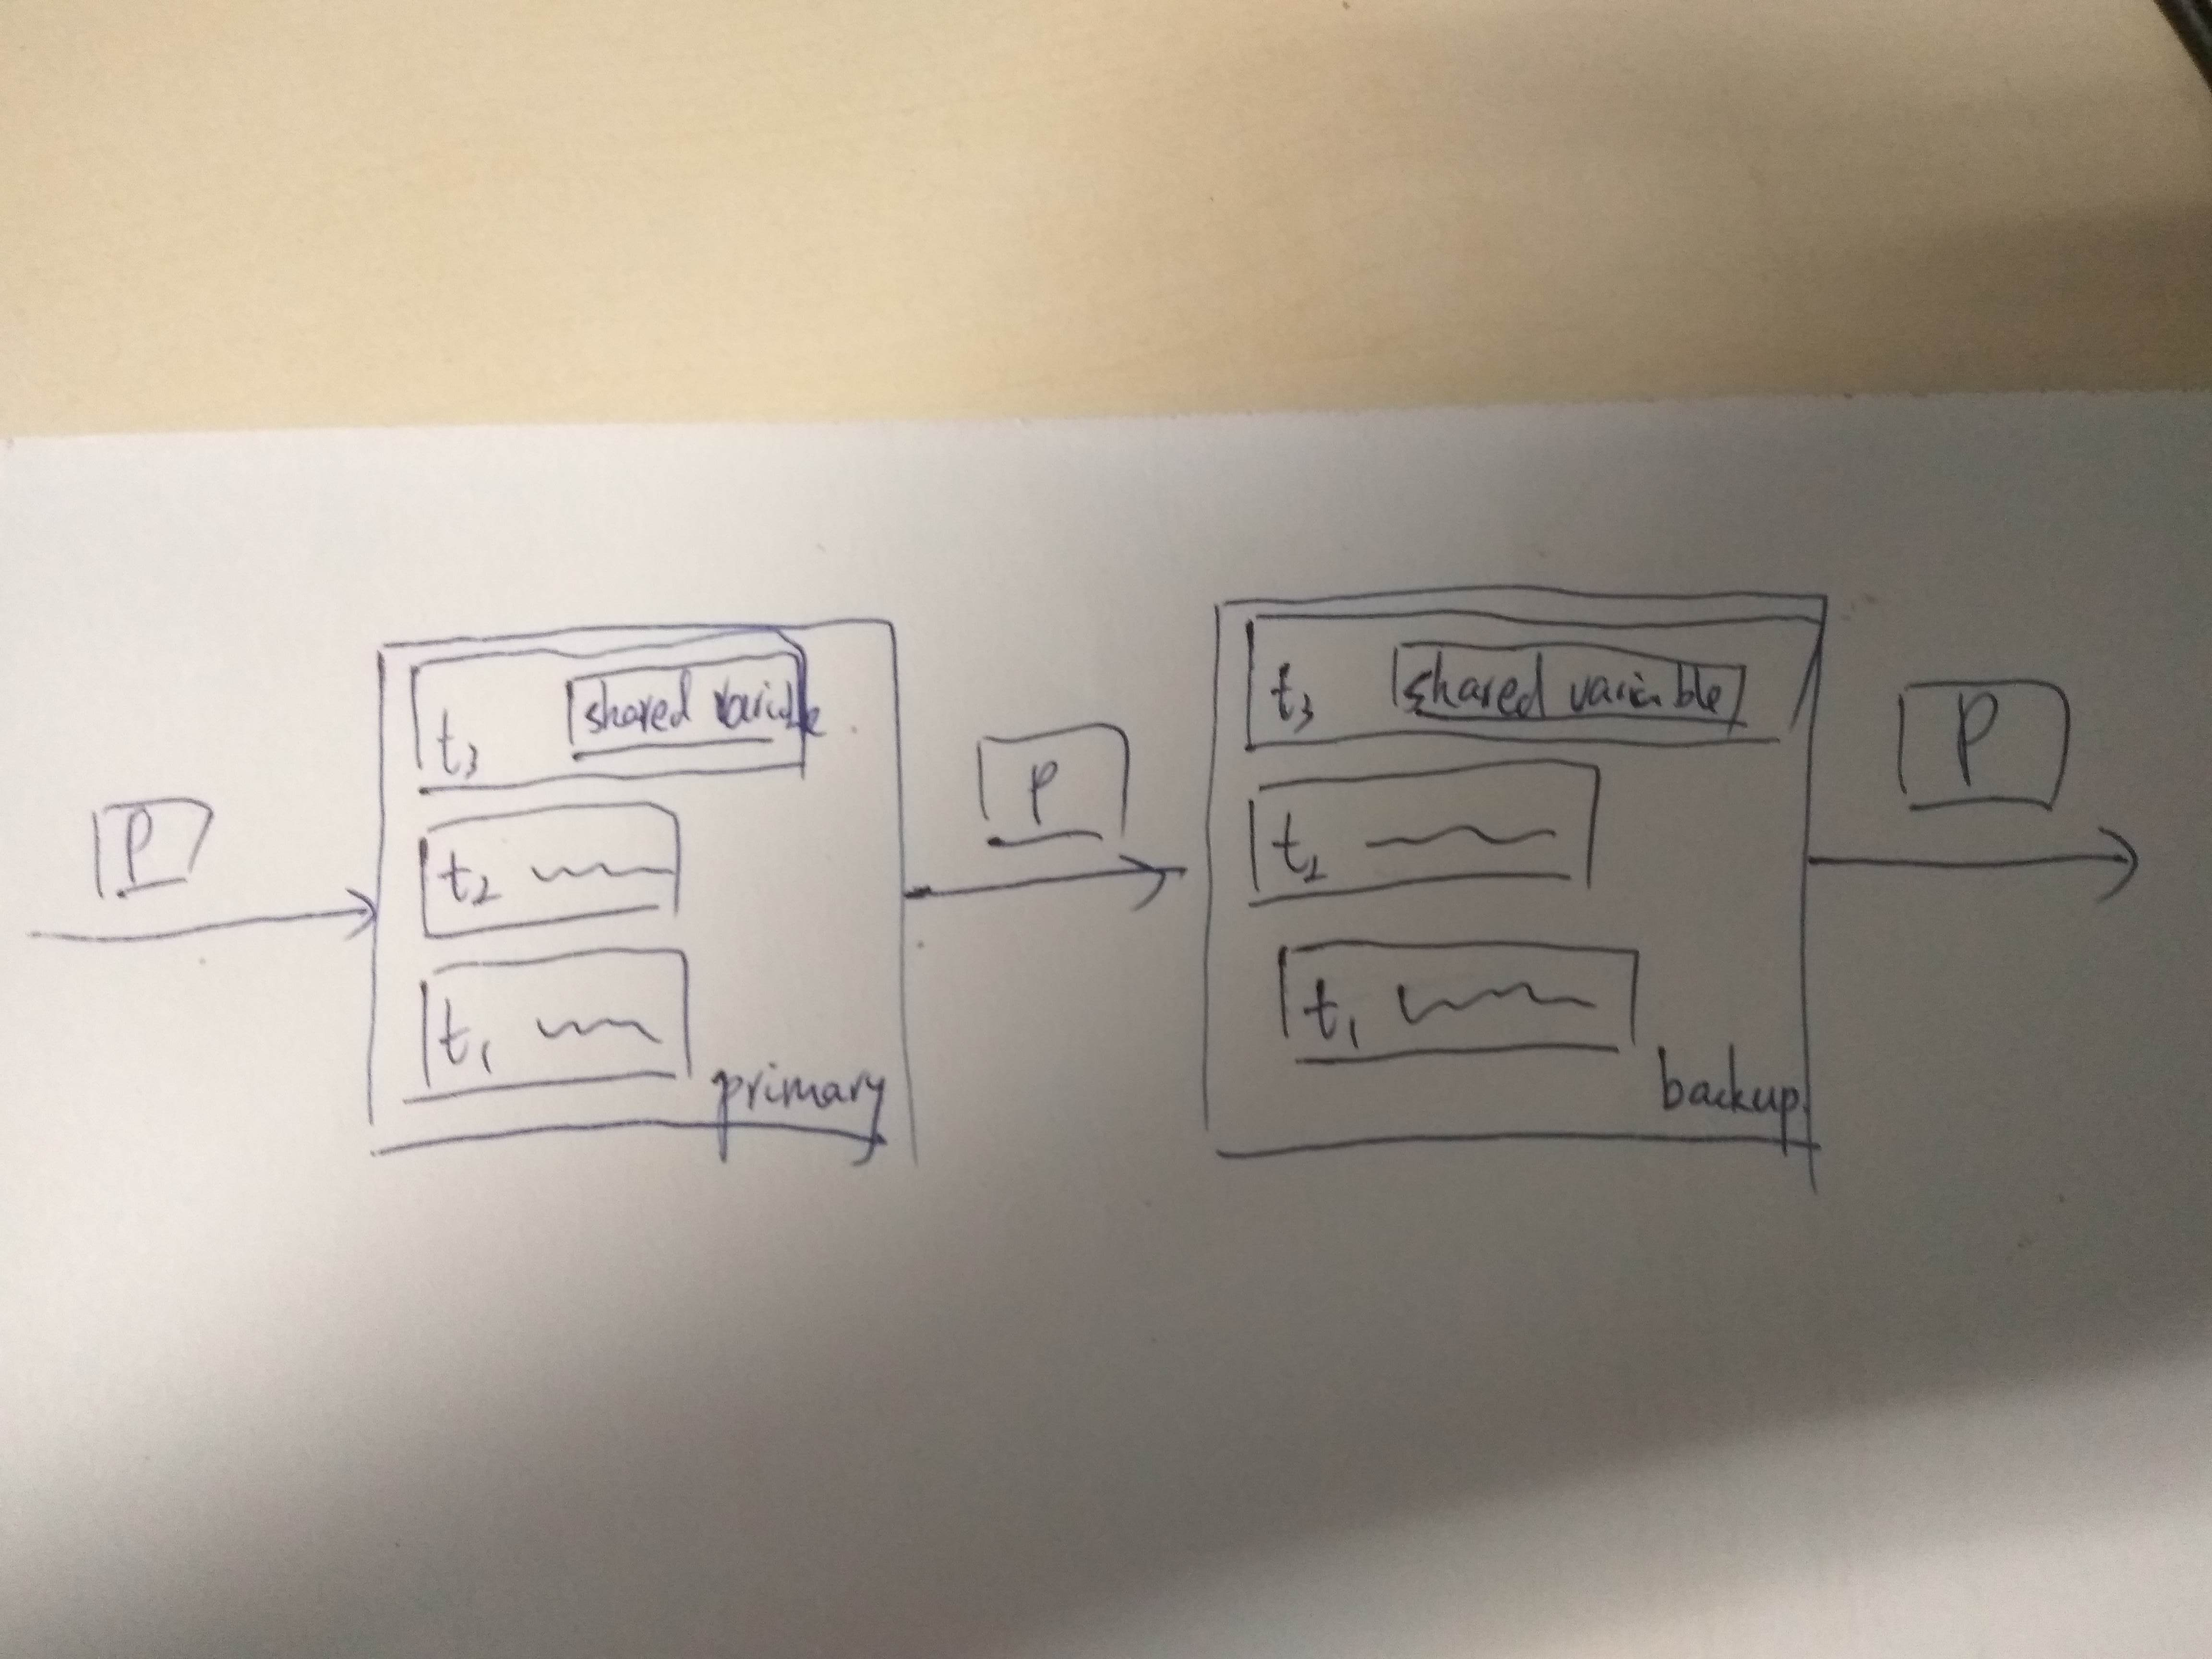
\includegraphics[width=\columnwidth]{section/overall.jpg}
    \resizebox{0.95\columnwidth}{!}{\theverbbox}
    \caption{The basic setup.}\label{fig:overall}
  \end{subfigure}\hfill
  \begin{subfigure}[t]{0.5\linewidth}
    \centering
    %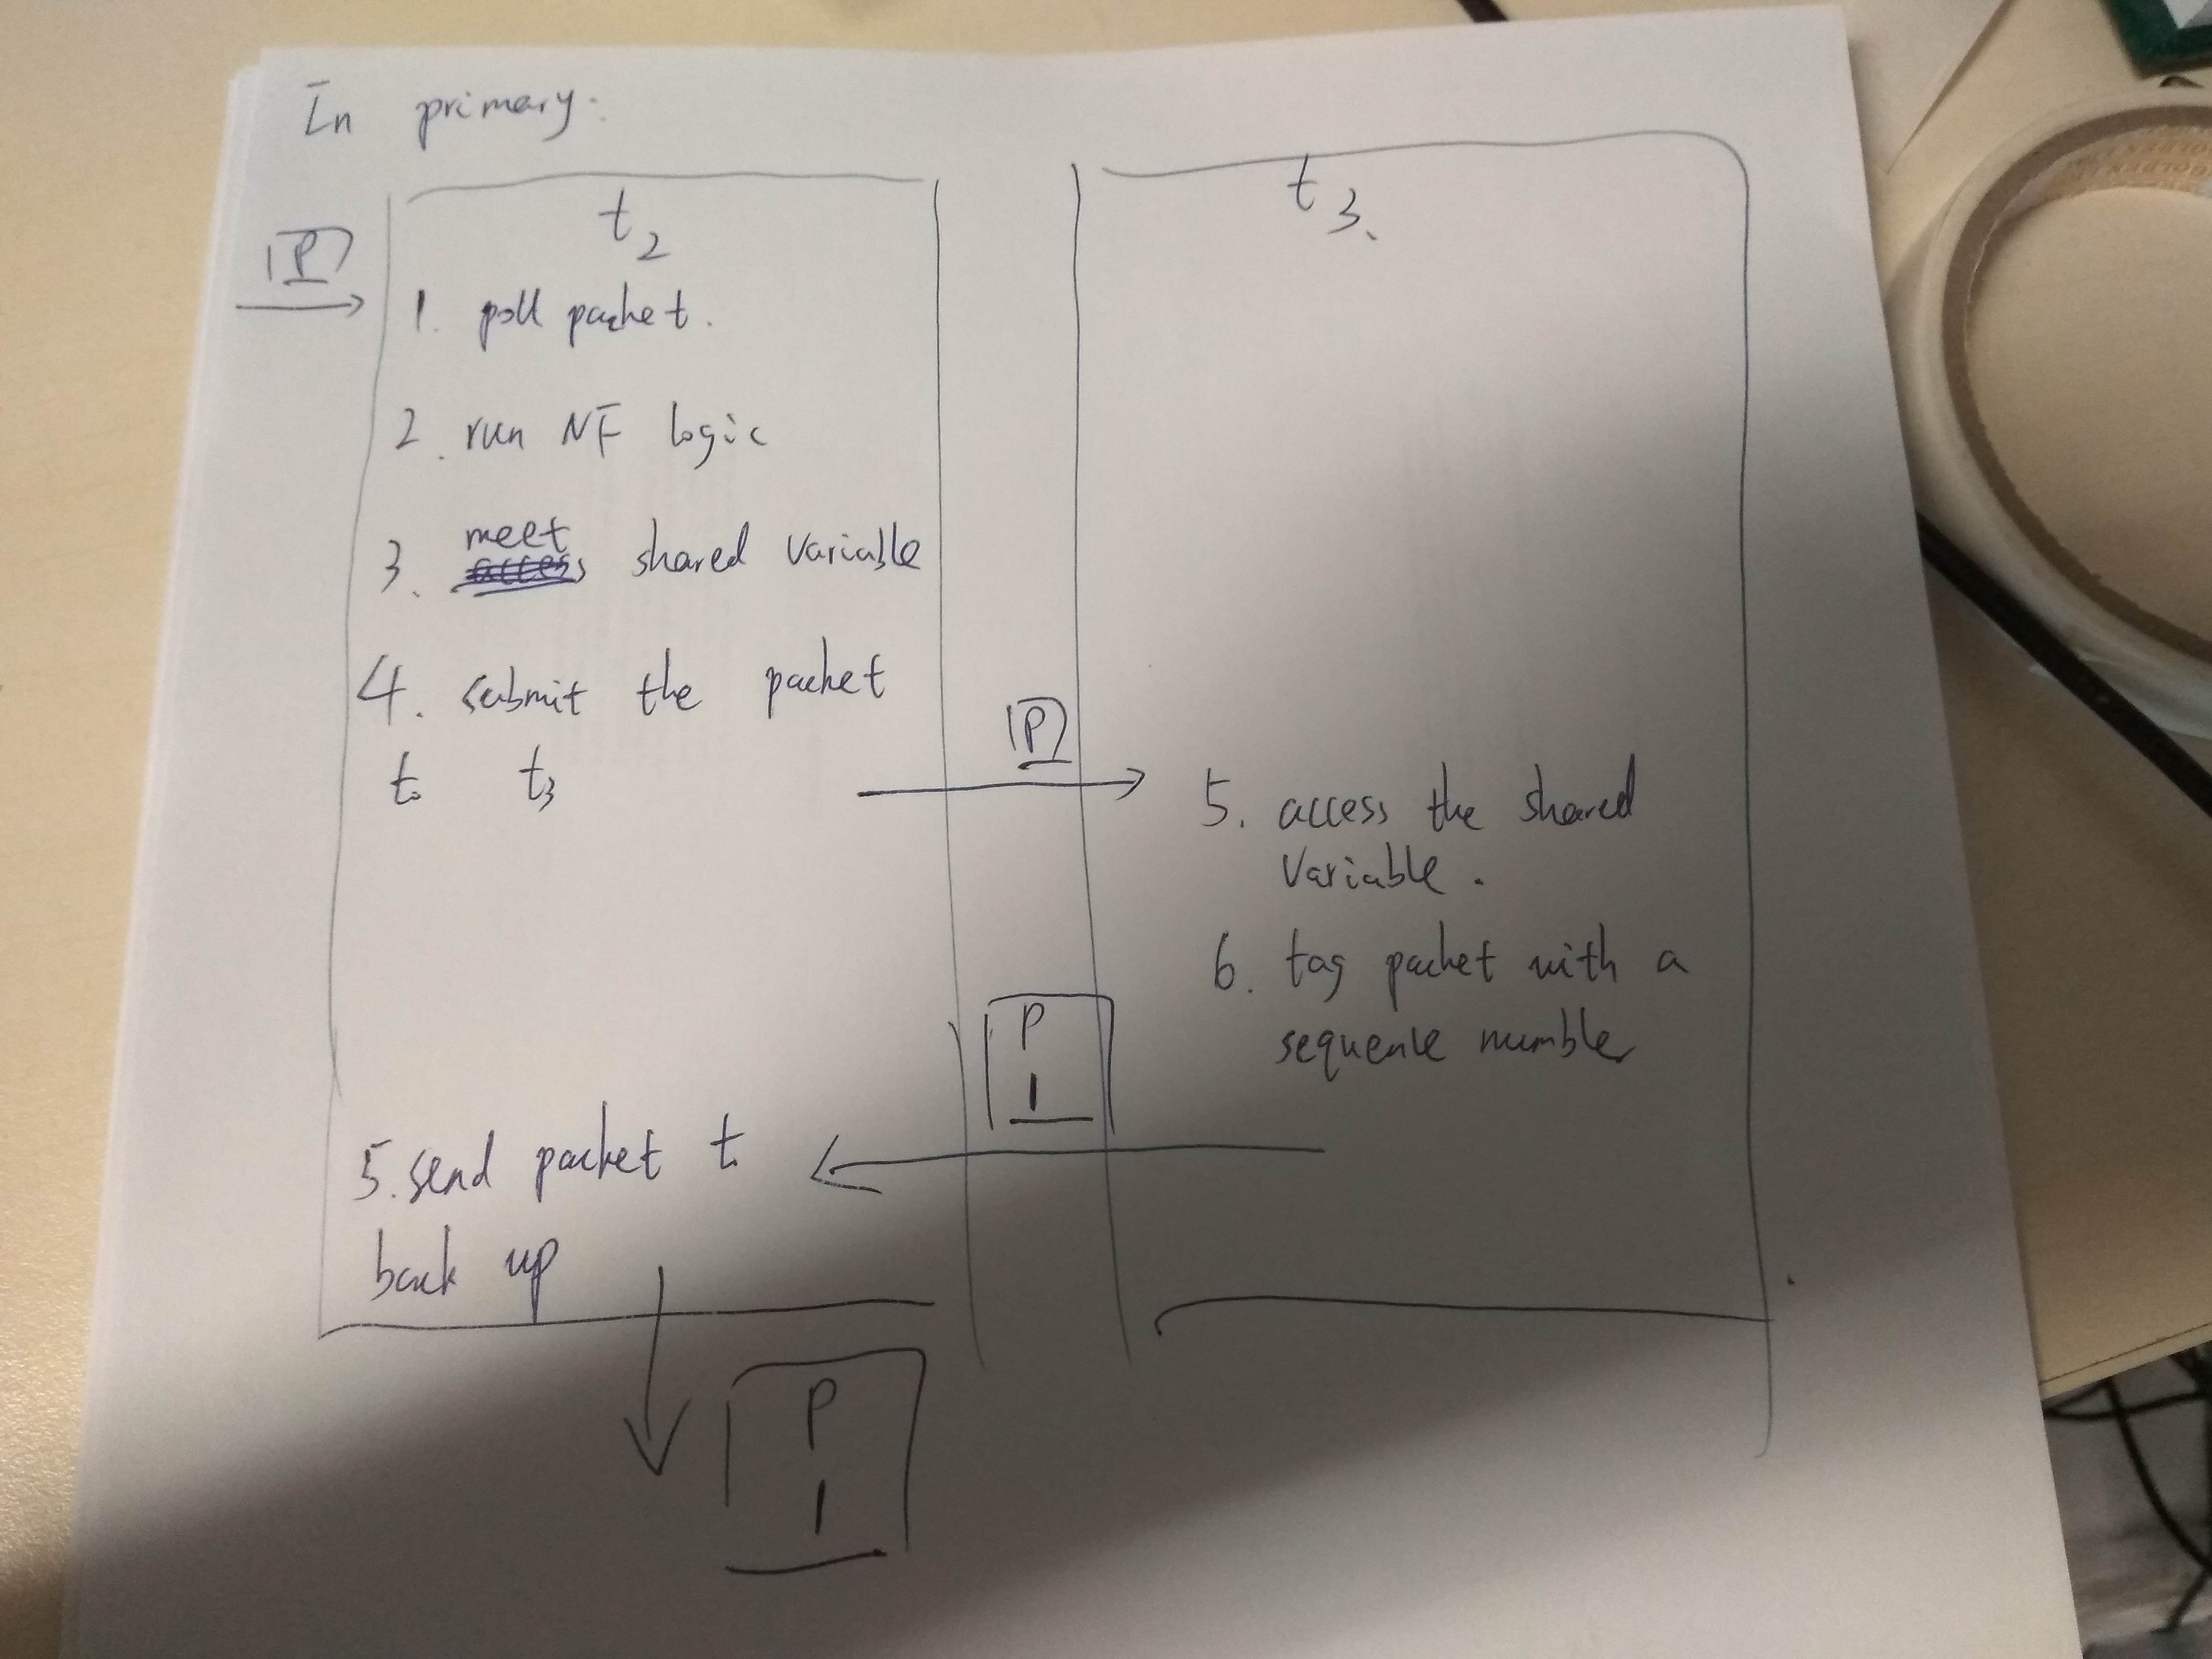
\includegraphics[width=\columnwidth]{section/primary.jpg}
    \resizebox{0.95\columnwidth}{!}{\theverbbox}
    \caption{The execution flow on a primary instance.}\label{fig:primary}
  \end{subfigure}\hfill
  \begin{subfigure}[t]{0.5\linewidth}
    \centering
    %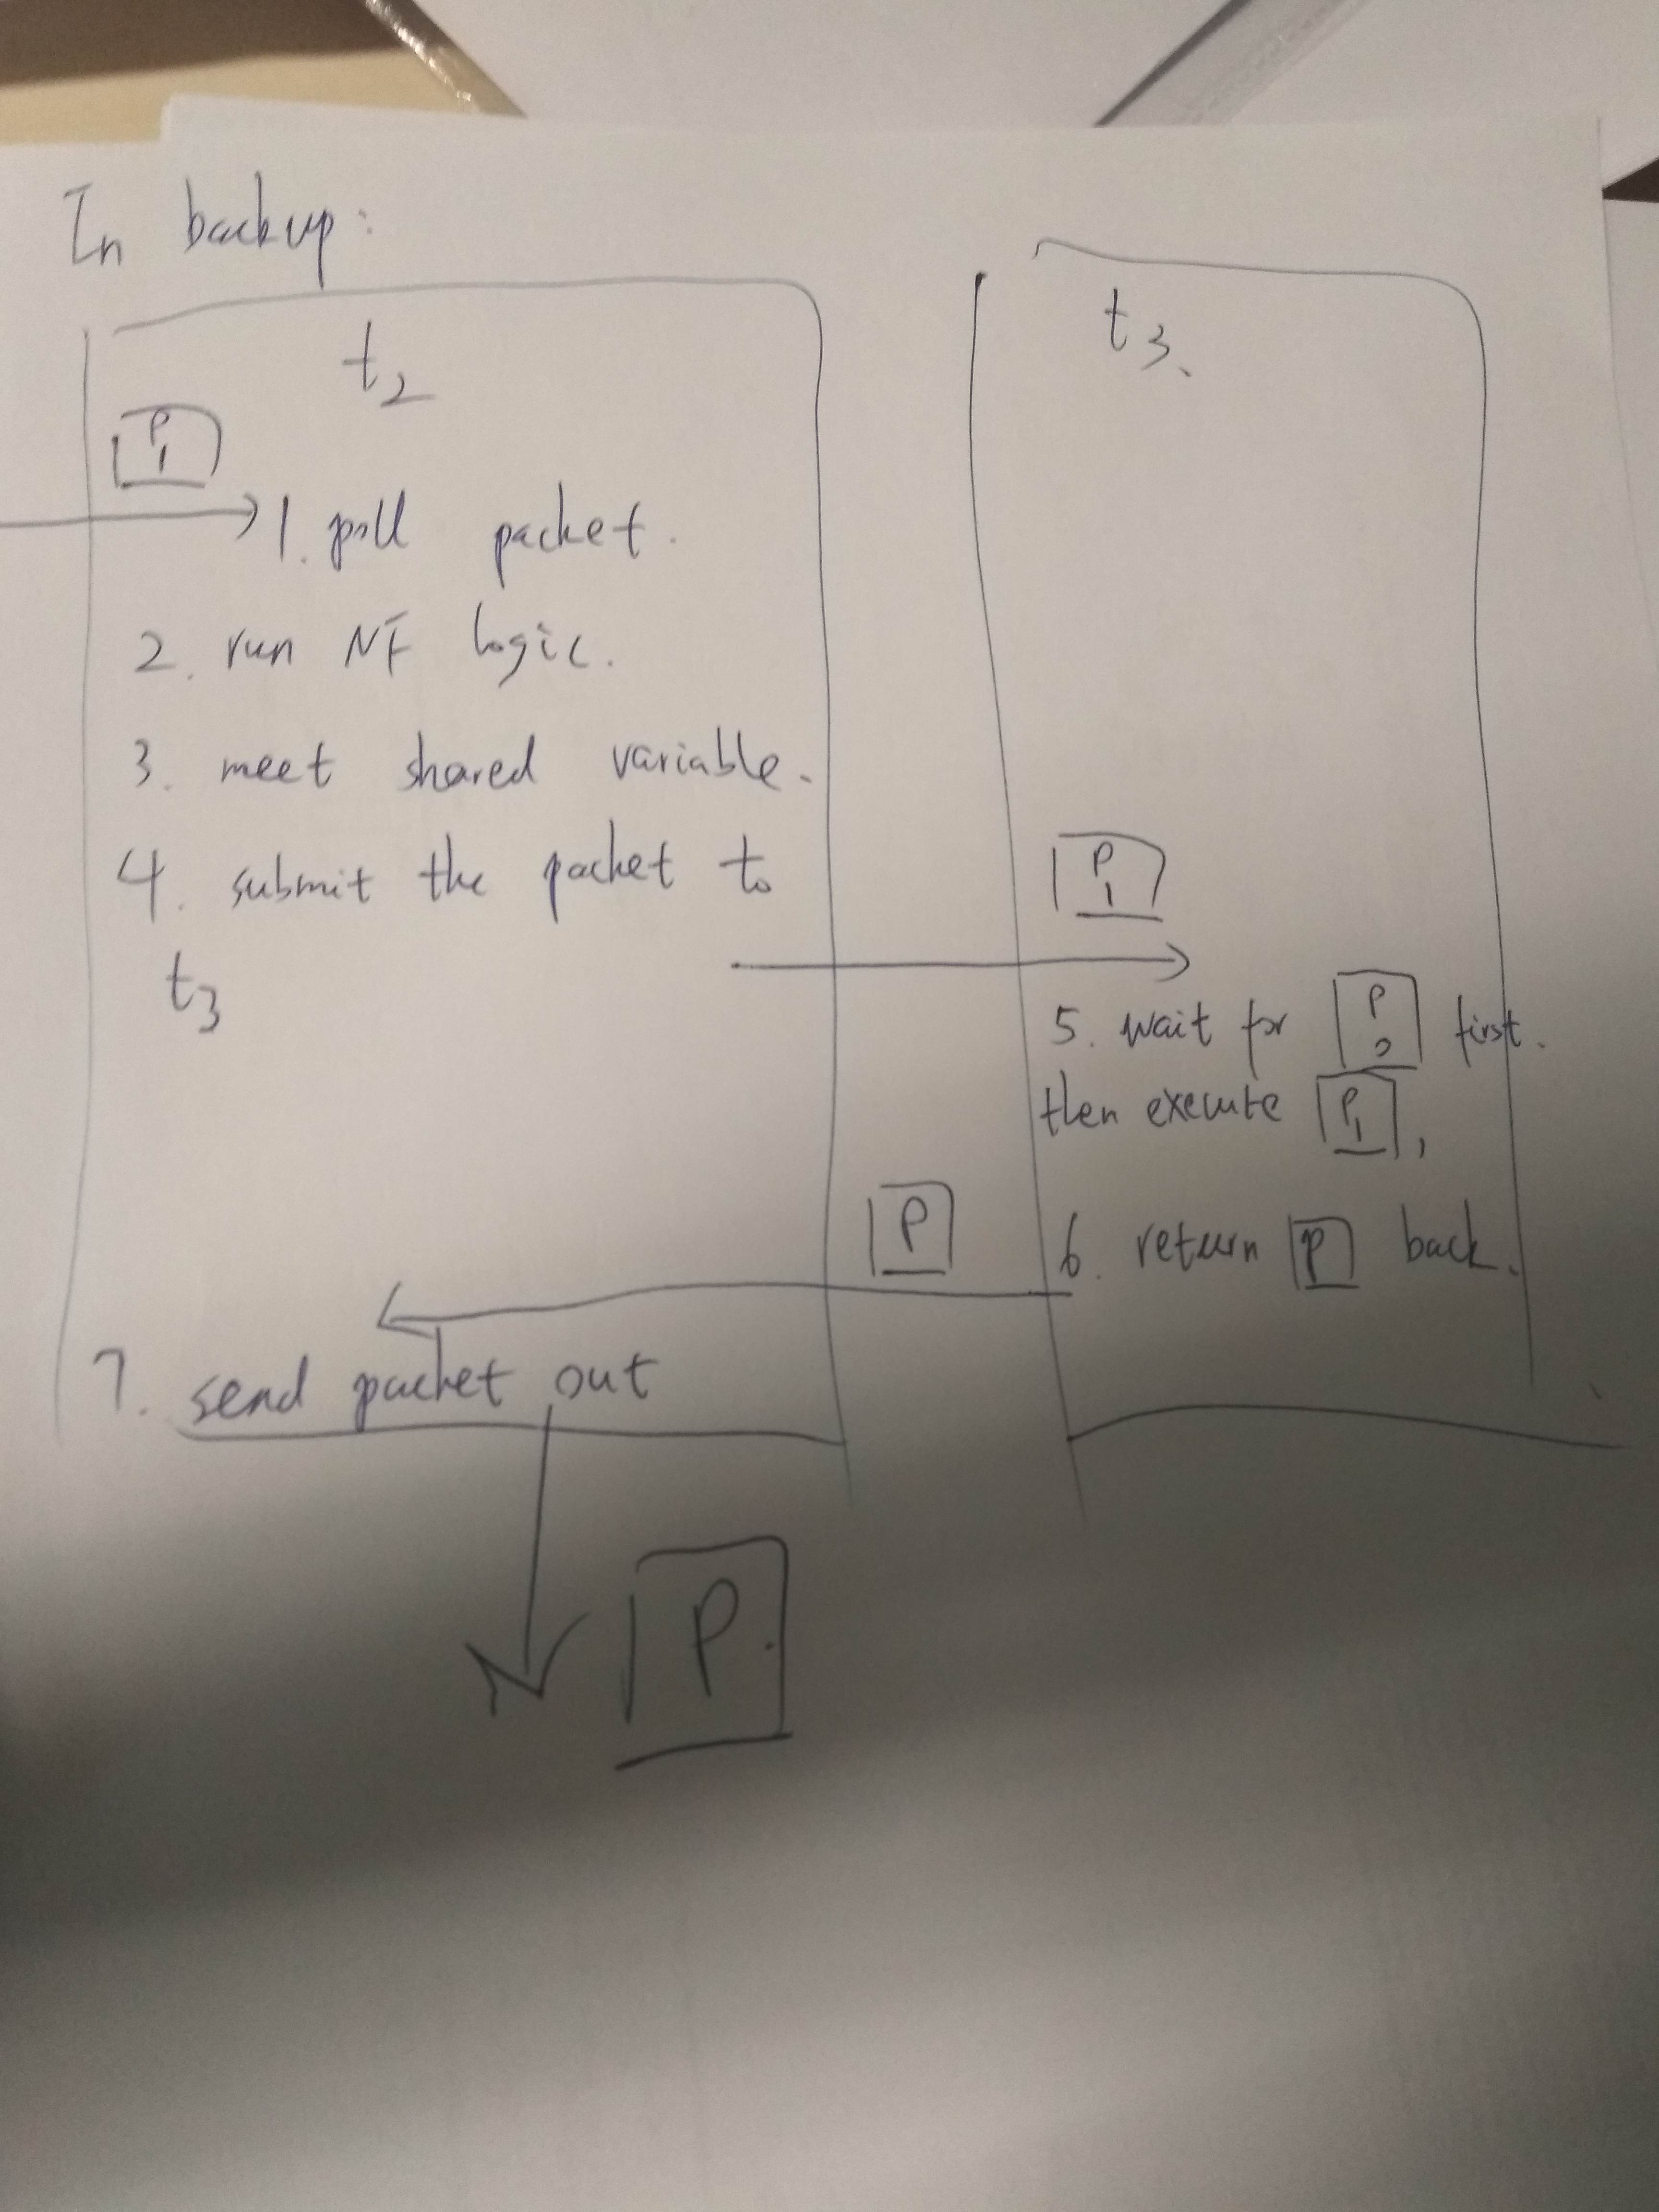
\includegraphics[width=\columnwidth]{section/backup.jpg}
    \resizebox{0.95\columnwidth}{!}{\theverbbox}
    \caption{The execution flow on a backup instance.}\label{fig:backup}
  \end{subfigure}
%Removed for better illustration.
\caption{Work flow of how to keep both primary and backup in synchronization.}
\label{fig:fig}
\end{figure}

\subsection{Basic Setup for Recovery without Rolling Back}

The basic setup is shown in figure \ref{fig:overall}. We set up two identical NF
instances. The two instances run the same NF software binary image and are
configured with the same number of CPU cores.

In \ref{fig:overall}, the NF instance is configured with two worker threads
($t_1$ and $t_2$) which poll the NIC card for input packet. The shared variable
is hosted on a dedicated thread $t_3$.

To access the shared variable hosted on $t_3$, both $t_1$ and $t_2$ need to send
a message for accessing the shared variable to $t_3$. After the shared variable
is modified, another message is sent back to $t_1$ or $t_2$ to indicate the
completion of shared variable modification.

When the primary instance finishes processing the input packet, it forwards the
input packet to the backup instance over a reliable communication channel. The
backup instance processes the input packet again before releasing the
packet. The packet processed by the backup instance is tagged with an execution
order by the primary, so that the shared variable on the backup instance can
process the input packet in the same sequence as the primary instance. This
guarantees that the state of both the primary instance and the backup instance
are always synchronized.

\subsection{Workflow on Primary Instance}

Figure \ref{fig:primary} shows how worker thread $t_2$ processes an input
packet. The overall workflow is similar to a typical packet polling loop. The
only exception is that when a shared variable is going to be accessed by $t_2$
(step 3 in figure \ref{fig:primary}), instead of directly acquiring the lock and
update the shared variable, $t_2$ sends the packet to $t_3$ to update the shared
variabale (step 4). When $t_3$ receives this packet, the threads update the
shared variable (step 5), tags the packet with a sequence number (step 6) and
sends the packet back to $t_2$. When $t_2$ receives this packet, $t_2$ sends the
tagged packet out to the backup instance over a reliable communication channel.

\subsubsection{The Sequence Number}

The sequence number tagged by $t_3$ indicates a sequential accessing order to
the shared variable. Using this sequence number, the backup instance can
reliably reproduce the accessing order of the shared variable (to be discussed
in section \ref{sec:backup}). This ensures that the state of the primary and backup
instances are always synchronized.

\subsubsection{Using Future and Promise to Cancel Thread Blocking}

The biggest problem with this workflow is that, after step 4 in figure
\ref{fig:primary}, worker thread $t_2$ must block its execution and wait for the
packet to come back from $t_3$. This is unacceptable for a high-performance NF
software.

We tackle this problem using futures and promises in reactive
programming. After step 4 in figure \ref{fig:primary} is executed, we wrap the
current thread context inside a future object. $t_2$ can immediately start processing
other input packets. When the packet comes back to $t_2$ after step
6, $t_2$ is able to re-construct the previous thread context using the
corresponding future object. This efficiently eliminates thread blocking.

\subsubsection{The Reliable Communication Channel}

Due to the power of future and promise, a user-space TCP/IP stack could be
integrated inside $t_2$. The reliable communication channel is actually a TCP
connection channel. This reliable communication channel is augmented with flow
control and is more reliable than other specially-crafted reliable communication protocols. 

\subsection {Workflow on Backup Instance}
\label{sec:backup}

Figure \ref{fig:backup} shows how worker thread $t_2$ processes the output
packet sent from the primary instance. The overall workflow is similar to that
of the primary instance. However, when the packet is delivered to $t_3$ to
access the shared variable, $t_3$ must check whether it has processed all the
packets whose sequence number is smaller than the packet. Considering the case
of figure \ref{fig:backup}, $t_3$ must wait for packet with sequence number 0
first. If $t_3$ has processed packet with sequence number 0, $t_3$ can directly
process the packet with sequence number 1. Otherwise, $t_3$ should store packet with
sequnece number 1 and wait for the packet with sequenece number 0 to come.

Since the order of how packets access the shared variable is well preserved,
the backup instance and the primary instance have the same state.

\subsection{Recovery}

If the primary instance fails, the backup instance can become the primary
instance immediately. The recovery time is basically decreased to zero.






%\section{Asynchronous Programming}
%The core idea of asynchronous programming is to handle all the tasks that need
%to block waiting for results asynchronously, so that nothing is really blocked.

%It can be implemented using an active poll loop. The active poll loop polls
%different event source for events. Whenever an event happens, the poll loop
%executes a callback function associated with the event to handle the event.

%An improved asynchronous programming style is to use futures and promises. The
%future and promise abstraction can handle asynchronous programming in a nice
%manner.

%Asynchronous programming is the solution for all the problems that I have
%mentioned in the previous section.

%\section{Seastar and OSv}

%Seastar is a modern asynchronous programming library with future and promise
%style. It can be combined together with DPDK to achieve low-level packets
%processing. It also includes a user-space TCP/IP stack that is driven by
%asynchronous programming.

%It is the best asynchronous programming library that we can use to build network
%functions.

%Seastar can also run in OSv, a unikernel. In this way we can achieve
%high-performance virtualization.

%\section{Planned Roadmap}

%I plan to do the following case studies using Seastar in this work.

%First, implementing an unified NFV platform like NetBricks. Highlight that with
%the help of C++ unique\_ptrs, we can achieve the similar software memory safety
%like NetBricks.

%Second, port PRADS to use Seastar. Show that with the help of asynchronous
%programming, we can greatly improve the performance of PRADS.

%Third, implement a simplified version of mOS. Show that asynchronous programming
%can greatly simplify flow event generation and processing.

%Fourth, re-implement FTMB. Show that how easy it is to implement primary-backup
%replication for network functions using seastar.

%Fifth, a simplified SDN switch using Seastar, show it's performance boost when
%compared against OpenVSwitch.

\section{Promises and Cooperative Threads}

In this section, I will first give a detailed overview about promises and
cooperative threads used by Seastar fraemwork. Then I will introduce how to
apply promises and coopeartive threads to NFV.

\subsection{Lwt}

The core building blocks of Seastar are promises and cooperative
threads. Clearly, these fancy concepts come from the world of functional
programming languages. There is an Ocaml library called Lwt \cite{vouillon2008lwt}, which also
implements promises and cooperative threads. In the following sections, I will
first discuss how promises and coopeartive threads are implemented in
Ocaml. Then I will show how they are implemented in Seastar.

\subsubsection{Lwt Overview}

When wring programs like network servers, non-blocking is a very important
property that ensures the runtime efficiency of the network servers. There are
two dominant techniques to make the program non-blocking. The first one uses
multi-threading to support non-blocking, i.e. whenever a blocking operation is
going to be made, the main thread of the program lanuches another thread to
handle the blocking operation. The second one uses event-based programming
method, i.e. the main thread treats the completion of the blocking operation as
an event and register corresponding event handlers to handle this event.

The first technique is easy to use and easy to program. The program can be
written in traditonal way without relying on callbacks. However, the first
technique lacks efficiency, as launching too many threads compromises the
runtime performance. On the other hand, the second technique has superior
runtime performance, as it only maintains a single thread. However, it is
difficult to write programs using the second technique due to excessive use of
callbacks.

Lwt uses promises and cooperative threads to support non-blocking. The runtime
performance of Lwt is very good, as it only maintains a single physical thread
like the second technique. And it is quite easy to use. Writing asynchrounous,
fully non-blocking programs using Lwt is just like writing synchronous, blocking
programs using the first technique.

%\verb!sdfs\_dff!

%\begin{verbatim}
%Text enclosed inside environment
%is printed directly
%and all \LaTeX{} commands are ignored.
%\end{verbatim}

In the following sections, to facilitate understanding, I simplify some concepts
related with exception handling and modify the name of some important types in
Lwt.

\subsubsection{Promise State}

\begin{figure}[!h]
        \centering
        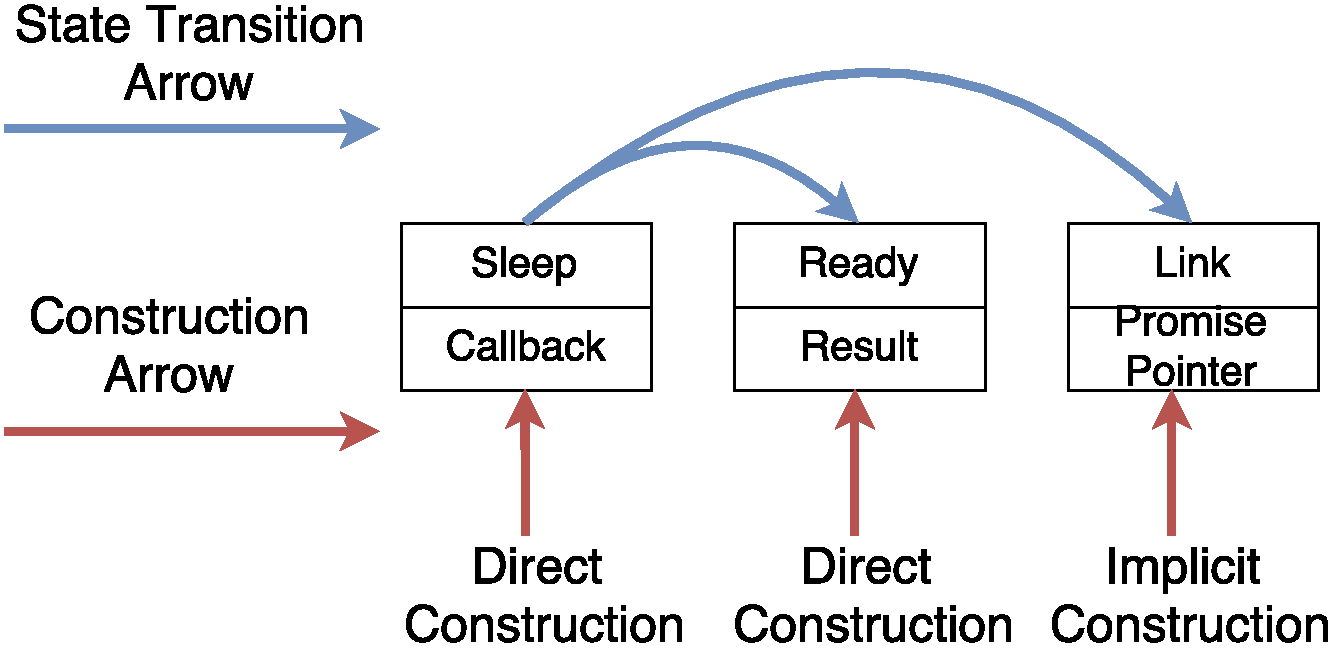
\includegraphics[width=1\columnwidth]{figure/promise-state.pdf}
        \caption{The state of a promise. The blue arrow represents how future
          states are transitioned. The red arrow represens whether can a
          programmer construct a certain state.}
        \label{fig:promise-state}
\end{figure}

The basic building block in Lwt is promise. A promise, as shown in figure
\ref{fig:promise-state}, has three states, which are \textbf{Sleep} state,
\textbf{Ready} state and \textbf{Link} state. The \textbf{Sleep} state
represents that the result of the promise is not available yet and one has to
wait before the \textbf{Sleep} state transitions into \textbf{Ready} state. The
\textbf{Sleep} state promise may contain a callback function, which is
immediately called after it is transitioned to \textbf{Ready}
state. \textbf{Ready} state represents that the result is available and we can
peek the result by checking the result field. Finally, the \textbf{Link} state
contains a pointer to a promise that is in \textbf{Sleep} state. It is used to
when waiting for multiple events.

The state of a proimse can be changed. The blue arrow of figure
\ref{fig:promise-state} shows the state transition graph between the three
states. Only \textbf{Sleep} state can generate a state transition.

When programming with promises, the programmer can only construct \textbf{Sleep}
state promise and \textbf{Ready} state promise. The \textbf{Link} state promise
is implicited constructed when chaining a promise with an annoynamous function
(we omit the discussion, as it does not affect the understanding of how promises
work).

\subsubsection{Chaining Promises}

\begin{verbbox}(>>=) : Promise a -> (a -> Promise b) -> Promise b \end{verbbox}

\begin{figure}[!h]
\resizebox{0.95\columnwidth}{!}{\theverbbox}
\caption{The infix operator for chaining promises.}
\label{fig:infix}
\end{figure}



Multiple promises can be chained together to accomplish complicated
tasks. Chaining is done through an infix operator \verb!>>=! (the then member
function of future in Seastar) as shown in figure \ref{fig:infix}, whose
signature is listed below.

Here, \verb!Promise a! represents a promise that, when transitioning into
\textbf{Ready} state, contains a result field with type \verb!a!. \verb!(a -> Promise b)!
represents an annouymous function, that takes a value of type \verb!a! as
argument and returns a value with type \verb!Promise b!. \verb!>>=! is a
function, that takes a value of \verb!Promise a! and an anouymous function of
\verb!(a -> Promise b)! and returns a value of \verb!Promise b!.

The real power of the \verb!>>=! operator is to chain multiple promises together
into a complicated operation. We give a piece of example code in figure
\ref{fig:example}. The code will first sleep for 3 seconds, then print "first
print" on the screen, then sleep another 3 seconds, and finally print "second
print" on the scrren. The best thing about this code is that, even if it
represents the consecutive execution of four blocking operations, but the code
itself is not blocking at all. It will return a promise in \textbf{Sleep} state
after being called. The blocking operations are implicitly handled by a
background thread.

\begin{verbbox}
  sleep 3 >>=
  fun () -> async_print "first print" >>=
  fun () -> sleep 3 >>=
  fun () -> async_print "second print"
\end{verbbox}

\begin{figure}[!h]
\resizebox{0.95\columnwidth}{!}{\theverbbox}
\caption{Chaining multiple promises into a complicated operation. The code above
  will first sleep for 3 seconds, then print "first print" on the screen, then
  sleep another 3 seconds, and finally print "second print" on the scrren.} 
\label{fig:example}
\end{figure}

\subsubsection{Annatomy of the infix operator}

\begin{verbbox}
(>>=) x f =
  match x with
  | Result r -> f r
  | Sleep ->
    let res = make_Sleep_promise () in
    add_callback x ( fun x -> connect res (x >>= f) )
    res
  | Link p ->
    assert false

connect t t' =
  match t' with
  | Result r -> (run t's callback)
  | Sleep ->
    (let t' link to t)
  
\end{verbbox}
\begin{figure}[!h]
\resizebox{0.95\columnwidth}{!}{\theverbbox}
\caption{The implementation of the infix operator. } %Depending on the state of the
  %promise \verb!x!, \verb!>>=! steps into three branches. If \verb!x! is a
 %result promise, then the annoynamous function.}
\label{fig:infix-internal}
\end{figure}

\noindent \textbf{The internal of the infix operator.} Depending on the state of
promise \verb!x!, the infix operator may step into two branches. If \verb!x! is
in \textbf{Result} state, then the anonymous function is immediately
excuted. But if \verb!x! is in \textbf{Sleep} state, the operator first creates a new
promise \verb!res! in \textbf{Sleep} state. Then a callback is added to \verb!x!. When
\verb!x! becomes \textbf{Result} state, the callback function is called, which
connects \verb!res! and \verb!x >> f!. The \verb!connect! function means that
the state of promise \verb!t'! will be reflected in promise \verb!t!.

\noindent \textbf{A conceptual explanation.} When executing \verb!x >>= f!, if
\verb!x! is immediately available and in \textbf{Result} state, then the
execution of the anonymous function \verb!f! continues without any
interruption.

The tricky part comes when \verb!x! is in \textbf{Sleep} state. It implies that
the result of \verb!x! is going to be available in the future. To prevent the
infix operator from blocking, we construct a new \textbf{Sleep} state promise
\verb!res! and returns \verb!res! to the user. Apparently, \verb!res! should
reflect the actual result of \verb!x >>= f!. To achieve this, before returning
\verb!res! to the user, we add a callback function to \verb!x!, which manually
connect \verb!res! with \verb!x >>= f! when \verb!x! becomes ready. In this way,
we mannualy construct a fully non-blocking abstraction.


\subsubsection{Wake Up Sleep Promise}

If a promise is in \textbf{Sleep} state, it must be waken up in the future and
transform into \textbf{Result} state. This is done by an external polling thread
which polls asynchronous completion messages. If the blocking operation that a
\textbf{Sleep} promise waits for has completed, the corresponding promise is
waken up.

\subsection{Seastar}

Seastar is basically a re-implementation of lwt in C++. It differes from lwt:

\textit{First}, the infix operator \verb!>>=! that chains promises together becomes
\verb!then! member function.

\textit{Second}, Seastar introduces a new object called \verb!future!, which is actually
a pointer object to the underlying promise. The reason is that C++ has no
garbage collection and Seastar has to manually manage the the memory allocation
of the promise object. Currently, Seastar either allocates the promise object
directly on the heap, or captures the promise object inside the callback
function. Therefore, to query the promise, seastar creates a pointer object
future, which contains a pointer to the underlying promise object.


\subsection{Promises in NFV}

We use promises to hide any kind of blocking operations when processing
packets. We give some usage examples.

\subsubsection{Simple Packet Processing}

\begin{verbbox}
xxx.then([]{
  process packet;
  return new_future;
}).then([]{
  process packet;
  return new_future;
})
  
\end{verbbox}
\begin{figure}[!h]
\resizebox{0.5\columnwidth}{!}{\theverbbox}
\caption{Example code of a simple packet processing software.} 
\label{fig:spps}
\end{figure}

It is straightforward to implement a simple packet processing software using
promises, as shown in figure~\ref{fig:spps}. The multiple chained promises
represent multiple processing stages on a packet processing pipeline.

\subsubsection{Using Promises to Hide Blocking During File IO}

\begin{verbbox}
xxx.then([]{
  do file IO;
  return new_future;
}).then([]{
  resume packet processing;
  return new_future;
})
  
\end{verbbox}
\begin{figure}[!h]
\resizebox{0.5\columnwidth}{!}{\theverbbox}
\caption{Example code of a NF that performs file IO.} 
\label{fig:file-io}
\end{figure}

Figure \ref{fig:file-io} represents a NF that performs file IO in the middle of
packet processing. Previously, this incurs kernel context switches and blocking,
which may compromise the performance of the NF. But with promise, the kernel
context switches and blocking are hidden by the promises, making the entire
operation fully non-blocking.

After issuing \verb!do file IO!, the NF software can continue to process other
flows. When file IO finishes, the processing of the original packet that incur
the file IO is resumed. This can greatly boost the performance of NFs that need
to perform file IO, such as PRADs.

\subsubsection{Handling Shared Variable Accessing}

\begin{verbbox}
xxx.then([]{
  access shared variable;
  return new_future;
}).then([]{
  resume packet processing;
  return new_future;
})
  
\end{verbbox}
\begin{figure}[!h]
\resizebox{0.5\columnwidth}{!}{\theverbbox}
\caption{Example code of a NF that needs to access shared variable.} 
\label{fig:asv}
\end{figure}

Figure \ref{fig:asv} shows an example of how to use promise to handle shared
variable processing. After issuing \verb!access shared variable!, the processing
is temporarily suspended and a request is created and sent to another thread to
access the shared variable. After modifying the shared variable, the suspended
packet processing is resumed.

By using promises, we can effectively linearize shared variable
accessing. Therefore we can keep the primary NF instance and the backup NF
instance in the same state, which simplifies primary-backup replication even in
multi-threaded environment.



{\footnotesize \bibliographystyle{acm}
\bibliography{Bibliography}}


\end{document}






